\documentclass[conference]{IEEEtran}
\IEEEoverridecommandlockouts
% The preceding line is only needed to identify funding in the first footnote. If that is unneeded, please comment it out.
\usepackage{cite}
\usepackage{amsmath,amssymb,amsfonts}
\usepackage{graphicx}
\usepackage{textcomp}
\usepackage{xcolor}
\usepackage{algorithmic, algorithm}
\def\BibTeX{{\rm B\kern-.05em{\sc i\kern-.025em b}\kern-.08em
    T\kern-.1667em\lower.7ex\hbox{E}\kern-.125emX}}
\begin{document}

\title{ Sequential algorithm to split, merge and resplit multidimensional arrays }

\author{\IEEEauthorblockN{1\textsuperscript{st} Timothée Guédon}
\IEEEauthorblockA{\textit{Department of Computer Science and Software Engineering} \\
\textit{Concordia University}\\
Montreal, Quebec, Canada \\
t\_guedon@encs.concordia.ca}
\and
\IEEEauthorblockN{2\textsuperscript{nd} Tristan Glatard}
\IEEEauthorblockA{\textit{Department of Computer Science and Software Engineering} \\
\textit{Concordia University}\\
Montreal, Quebec, Canada \\
tristan.glatard@concordia.ca}
\and
\IEEEauthorblockN{3\textsuperscript{rd} Valérie Hayot-Sasson}
\IEEEauthorblockA{\textit{Department of Computer Science and Software Engineering} \\
\textit{Concordia University}\\
Montreal, Quebec, Canada \\
valerie.hayot-sasson@concordia.ca}
}

\maketitle

\begin{abstract}
% This document is a model and instructions for \LaTeX.
% This and the IEEEtran.cls file define the components of your paper [title, text, heads, etc.]. *CRITICAL: Do Not Use Symbols, Special Characters, Footnotes,
% or Math in Paper Title or Abstract.
\end{abstract}

\begin{IEEEkeywords}
multidimensional, array, split, merge, resplit, IO, processing, Dask, Python
\end{IEEEkeywords}

%----------------------------------------
\section*{Introduction}
%----------------------------------------

\subsection{Context}

With the improvement of aquisition methods in several scientific domains like health sciences, geology and astrophysics, processing a deluge of very high resolution images has become a Big Data challenge. Most pipelines process only specific ROI or process data by block. At the end of the pipeline, merging those blocks into one file may be required as well. Previous work in \cite{seqalgorithms} introduced two types of sequential algorithms to split and merge very high resolution images: the ``clustered" and ``multiple" strategies. In this paper, we define a new algorithm to resplit data that has already been splitted before into an other shape, and we show that it can also be used to split and merge data with the same behavior of the ``multiple" strategy. We also give an implementation of this algorithm, available as an optimization package for the Python big data library ``Dask".

\subsection{Problem definition}

Consider a multidimensional array of shape $R = (R_i, R_j, R_k)$, stored in some input files with a given shape $I = (I_i, I_j, I_k)$, all input files having the same shape.
Our goal is to optimize the process of sequentially resplitting the input files into output files with a different shape $O = (O_i, O_j, O_k)$, all output files having the same shape, too. \\

The resplit process has two particular cases:
\begin{itemize}
  \item It becomes a split process if there is one input file and several output files,
  \item It becomes a merge process if there are several input files and one output file.
\end{itemize}

For this I/O process to be fast, one needs to minimize the number of seeks that occur on disk while reading and writing.
We consider that a seek occurs either when opening a file or seeking into a file. \\

Let us consider a basic sequential resplit algorithm: One can repeatedly read the maximum amount of data possible from the input files into a buffer stored in main memory, and then write this buffer down into the output files requiring this data, until all output files have been completely written.
This resplit algorithm is described in Algorithm \ref{algo:generalresplit}. \\

The algorithm described in Algorithm \ref{algo:generalresplit} takes a list of input and output files $inFiles$ and $outFiles$ as parameters, as well as the amount of memory $m$ available in RAM for the buffer and the list of the buffers' coordinates. We call $m'$ the amount of memory available in the buffer at a given time during the execution of the algorithm ($m'=m$ at initialization). The list of buffers' coordinates contains the coordinates of each buffer to be loaded in the referential of the reconstructed image. \\

The algorithm successively loads as much data as it can from the input files into the buffer and write it down to the output files that are supposed to contain this data.
Although we could use a naive shape for the buffer, we can use the input and output files shapes to elaborate more efficient strategies as we will see in the next sections.
The algorithm ends when all buffers have been read.
Therefore, the buffers must cover the whole reconstructed image such that when the algorithm end all the output files have been completely written.
For the latter statement to be true, we also need to ensure that all data read from input files are either stored in RAM or directly written, such that all the output files are completely written at the end of the algorithm. \\

Given Algorithm \ref{algo:generalresplit}, the optimization problem that we want to solve can be stated as follows:
Given the amount of main memory available $m$, as well as the shapes of the input and output files $I$ and $O$, how to select the best buffer shape $B$ which will minimize the number of seeks that take place during reading and writing? \\

We add two restrictions on the buffers: We shall use only non-overlaping buffers, all buffers having the same size, and each buffer has to be written only once.

\begin{algorithm}[H]
  \caption{Basic resplit algorithm}
  \label{algo:generalresplit}
  \begin{algorithmic}
    \STATE \textbf{Inputs:} {inFiles, outFiles, m, buffersList}
    \FOR{$\textrm{buffer in buffersList}$}
      \STATE $\textrm{read(inFiles, buffer)}$
      \STATE $\textrm{write(outFiles, buffer)}$
    \ENDFOR

  \end{algorithmic}
\end{algorithm}

\subsection{Consistency with previous works}
For the sake of consistency with previous works \cite{seqalgorithms}, we call the original array of shape $R$ stored in the input files the ``reconstructed image" (see Figure \ref{fig:reconstructed_img_divided}).
Of course, the input files' positions in the reconstructed image have to be stored in some way.
Also with a view to be consistent with previous works, we assume the files to be written in column-order.
In column ordering (also called ``F" ordering) the fastest moving dimension is the last dimension of the array and the slowest moving dimension is the first dimension.
For example a 3D array with dimensions i, j and k would be written on disk by writing the complete columns in the k dimension first (see Figure \ref{fig:column_order}).

\begin{figure}[h!]
\centering
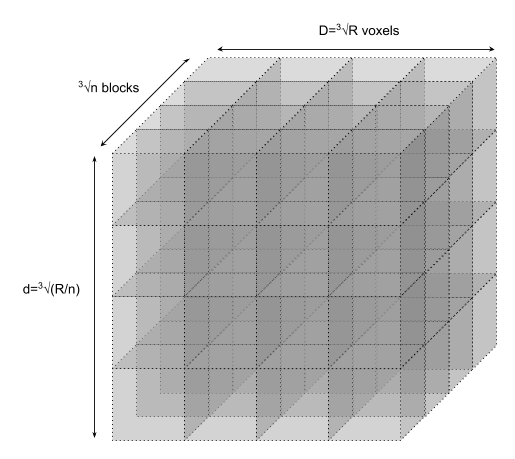
\includegraphics[scale=0.2]{./figures/reconstructed_img_divided.png}
\caption{Illustration of the reconstructed image divided into input files at the initialization of the resplit algorithm.
}
\label{fig:reconstructed_img_divided}
\end{figure}

\begin{figure*}[h!]
\centering
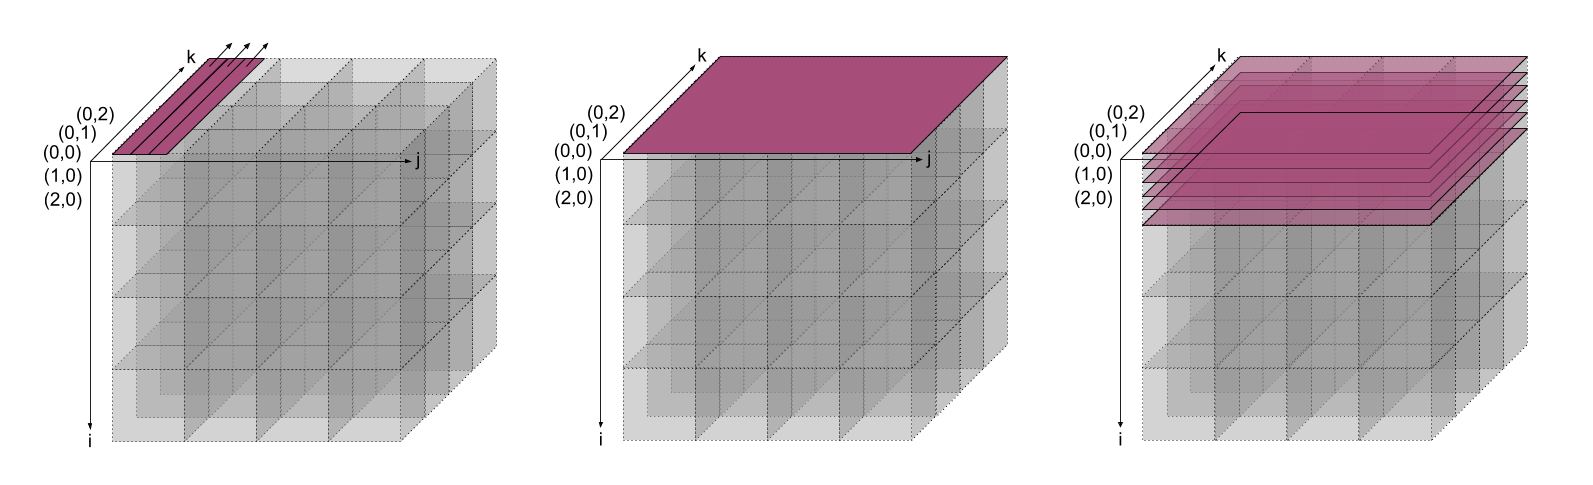
\includegraphics[scale=0.2]{./figures/column_order.png}
\caption{Illustration of the column-order storage of voxels in a file.
}
\label{fig:column_order}
\end{figure*}

\subsection{Naive algorithm}

As a base case for our problem, let us define a naive algorithm which loads one input file at a time and write it down into the different output files that requires the data.
The buffers have the same shape as the input files ($B=I$) and the order is the same order than the storage order i.e. the column order in this study ($[k, j, i]$ order).
% TODO : seeks analysis

\subsection{A particular case}

If the input shape is a multiple of the output shape such that one input file covers several output files entirely without falls, then the problem is easily solved: one must read as much input files as one, i.e. the buffer shape $B$ is a multiple of the input shape $I$.
The algorithm will produce one seek per input file and one seek to write each output file, which is the minimum number of seeks possible for a resplit.\\

If there is a mismatch between the shapes in any dimension however, one needs a strategy to manage with this overlap while minimizing the number of seeks.
We will introduce a strategy to keep falls temporarily into memory in the next section, this strategy's efficiency is completely dependent on the amount of main memory available. \\

Also, the resplit process requires multiple buffers to be read.
If there is no overlap between input and output files, then the order in which we load buffers is not important.
In case of an overlap however, the order may have an important impact on the number of seeks produced.

%----------------------------------------
\section*{The ``keep" algorithm}
%----------------------------------------
The algorithm presented in this paper is called the ``keep" algorithm, as it relies on a so-called ``keep strategy" that is presented below.

\subsection{The ``keep" strategy}
At initialization, we assign a shape $B = (0, 0,..., 0)$ for the buffer.
We will then stretch the buffer in each dimension until all the available memory $m$ has been used while keeping the number of seeks as small as possible. \\

Let us consider the first dimension $f$ that we increase: Ideally, one wants the buffer to cover both the input file and the output file, $I_f$ and $O_f$, such that we read and write in one seek each.
If there is a mismatch between $O_f$ and $I_f$ (meaning one is not a multiple of the other) we want to read a multiple of $O_f$ or $I_f$ such that we either read partially or write partially but not both at the same time.
We must therefore choose between reading a multiple of $O_f$ or $I_f$.
Reading a multiple of $I_f$ in the case of a shape mismatch is equivalent to $B_f = nI_f = mO_f+xO_f$ with $0<x<1$, $n$ and $m$ are integers.
We call ``extra data" the data contained in the overlap areas/volumes between input and output shapes (Figure \ref{fig:overlap}).
In this example the extra data is $xO_f$.
An output file that is involved in an overlap is called an ``incomplete output file". \\

\begin{figure}[h]
\centering
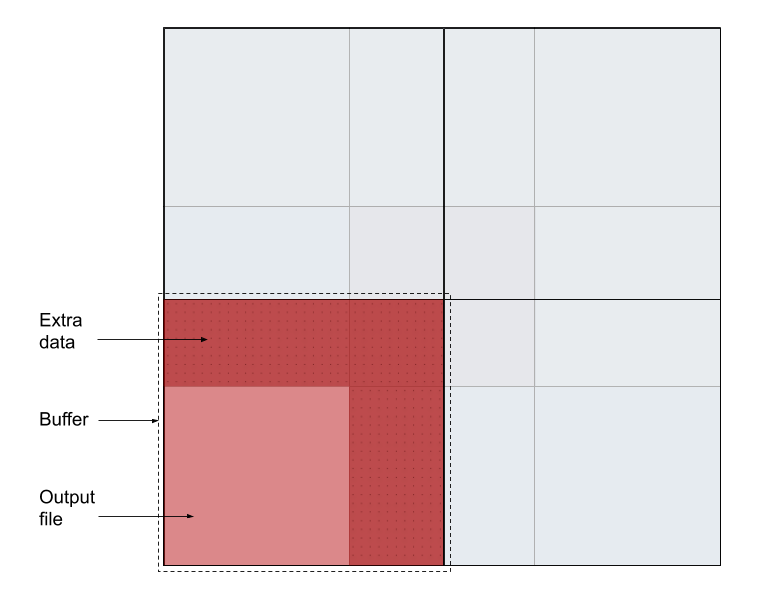
\includegraphics[scale=0.2]{./figures/overlap.png}
\caption{Illustration of the concept of extra data with a 2D case. In this example the black bordered rectangles represent the input files and the gray bordered rectangles represent the output files. After having read the red buffer we can see that the output file covered by the light red area can be written directly. After having written the data from the light red area however, we are left with the dark red, dotted area which represents some extra data we would like to keep in memory until we read the rest of the incomplete ouptut files in order to read the incomplete output files with one seek.
}
\label{fig:overlap}
\end{figure}

\begin{figure*}[h]
\centering
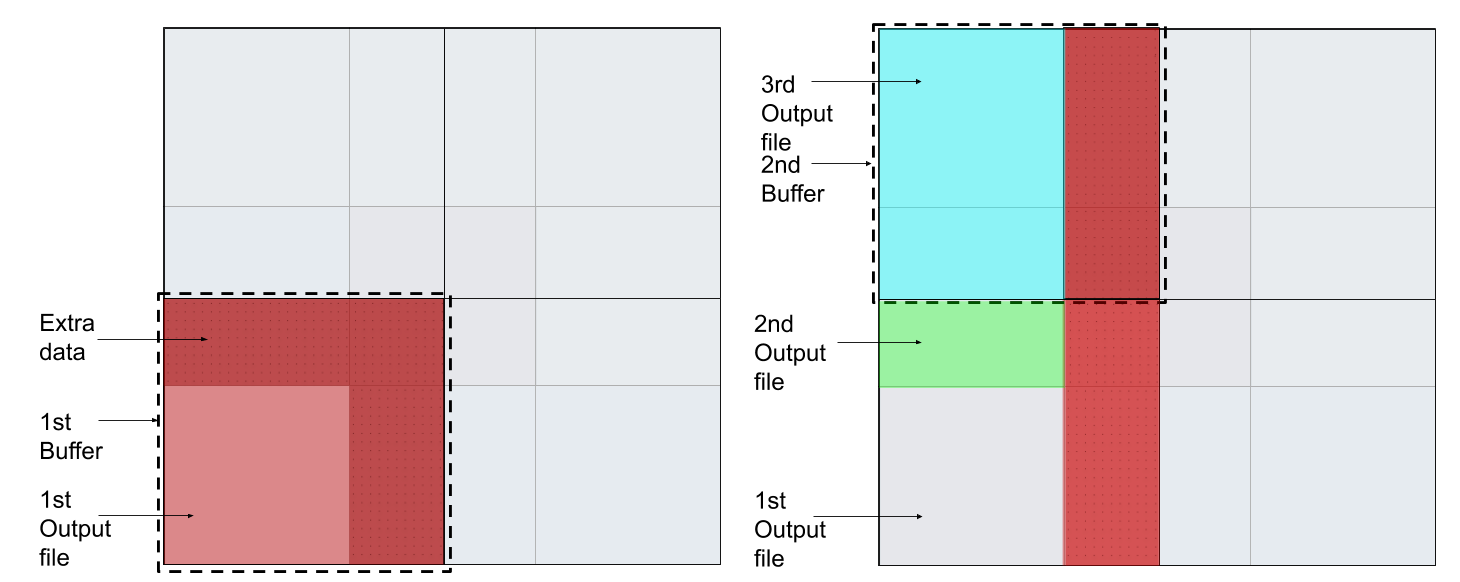
\includegraphics[scale=0.2]{./figures/keep_strategy.png}
\caption{Illustration of the keep strategy with a 2D case. In this example the black bordered rectangles represent the input files and the gray bordered rectangles represent the output files. As shown on the left figure, the keep strategy consists in reading more than one output file (light red area) into the first buffer. Then the first output file is written and the dark red area is kept in memory. On the left figure the second buffer has been loaded. It allows to free part of the overlap in the $k$ direction (the green area) as the second file data is complete in main memory. The third output file has been read completely and can therefore be written. This lets the overlap in the $j$ direction (dark red area) in main memory for the next buffer.
}
\label{fig:keepstrategy}
\end{figure*}

One can try to keep the extra data in memory instead of writing it directly into the output file: this is what we call the ``keep strategy" (Figure \ref{fig:keepstrategy}).
The idea is to read ``more than necessary" from the input files, ideally reading each input file in one seek, and to keep as much extra data in memory as possible.
The goal of this strategy is to read input files in one seek, and write as much output files as possible in one seek as well.
If we were to read a multiple of $O_f$ however, we would read an intput file partially and there is nothing that one can do about it.
It may be that we can only keep some of the overlaps in memory as it could take too much buffers until we can write an incomplete output file in one seek without running out of memory.
Extra data that cannot be kept in memory is written directly in the output file(s).
By doing so we ensure that when the algorithm ends all the data has successfully been written.

\subsection{Input and output aggregates}
We call ``input aggregate", $\Lambda$, the aggregate of the minimum number of input files that covers one output file entirely in all dimensions (see Figure \ref{fig:input_aggregates}, Figure \ref{fig:firstbuffer}).
The input aggregate is the minimal buffer shape we would like to have to be capable of minimizing the number of seeks as it allows to read the input files in one seek and to use the keep strategy.
The mismatch between the input and output shapes and the limited memory available for the buffer may prevent it to be possible. \\

\begin{figure}[h]
\centering
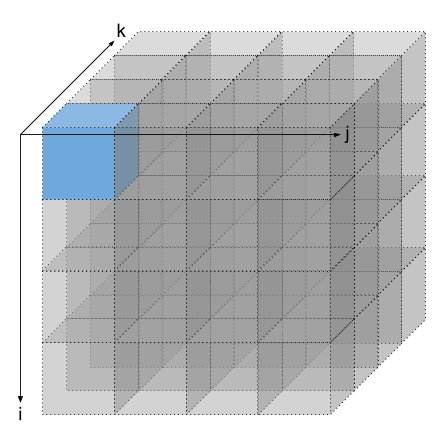
\includegraphics[scale=0.2]{./figures/first_buffer.png}
\caption{First buffer in the column-order storage.
}
\label{fig:firstbuffer}
\end{figure}

\begin{figure}[h]
\centering
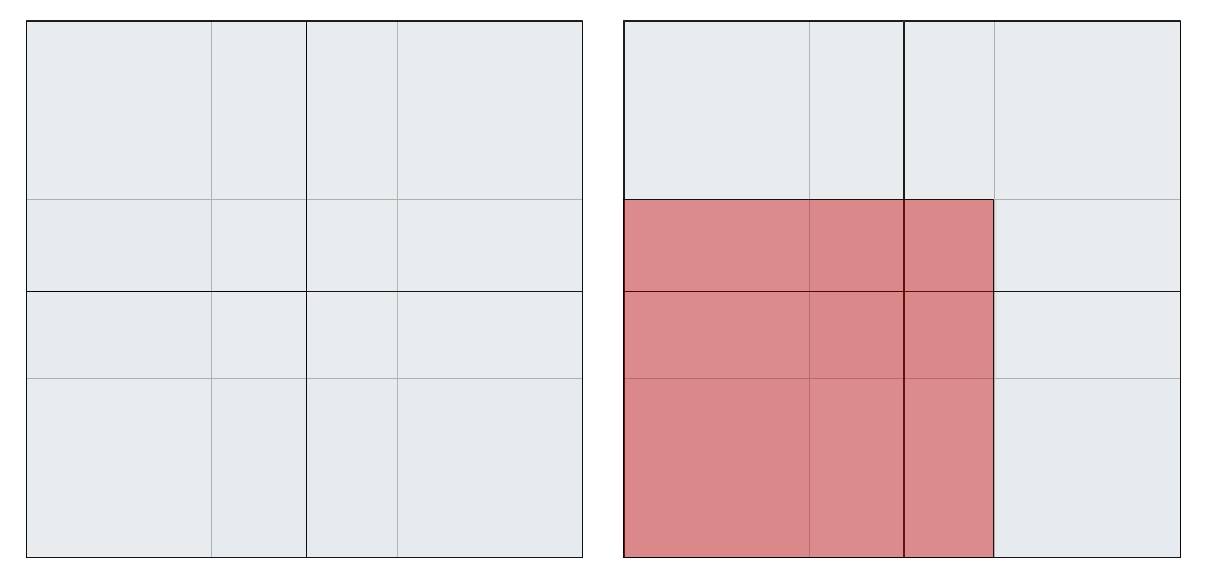
\includegraphics[scale=0.15]{./figures/input_aggregates.png}
\caption{Illustration of an input aggregate in two dimensions. On the left schema, consider the surface containing all rectangles as being the reconstructed image, with the small rectangles (with black borders) being the input files and the big rectangles (with gray borders) being the output files. On the right side an input aggregate is illustrated by the red area: it is the smallest number of input files such that the surface of at least one output file is completely covered. In this example, four input files are required to cover the first output file.
}
\label{fig:input_aggregates}
\end{figure}

We call ``output aggregate", $\Omega$, the aggregate of the output files that are being written by the $i^{th}$ buffer. It includes the incomplete output files for which the missing data have been loaded by the $i^{th}$ buffer. \\

\subsection{Stretching the buffer in the storage order}
The first step of the algorithm is therefore to make the dimensions of the buffer match the dimensions of the input aggregate as much as possible (we want $B=\Lambda$).
If more memory is available after that, we may want to increase the buffer's dimension even further (it is discussed in subsection ``Stretching beyond the input aggregate shape" below).
The question of which dimension should be increased first remains.
One should increase the buffer's dimensions in the order of the fastest moving dimensions.
For example if one is processing a 3D image stored in files following the column-order, one should increase the buffer in the $k$ dimension first, then the $j$ dimension and finally the $i$ dimension. \\

\begin{figure*}[h]
\centering
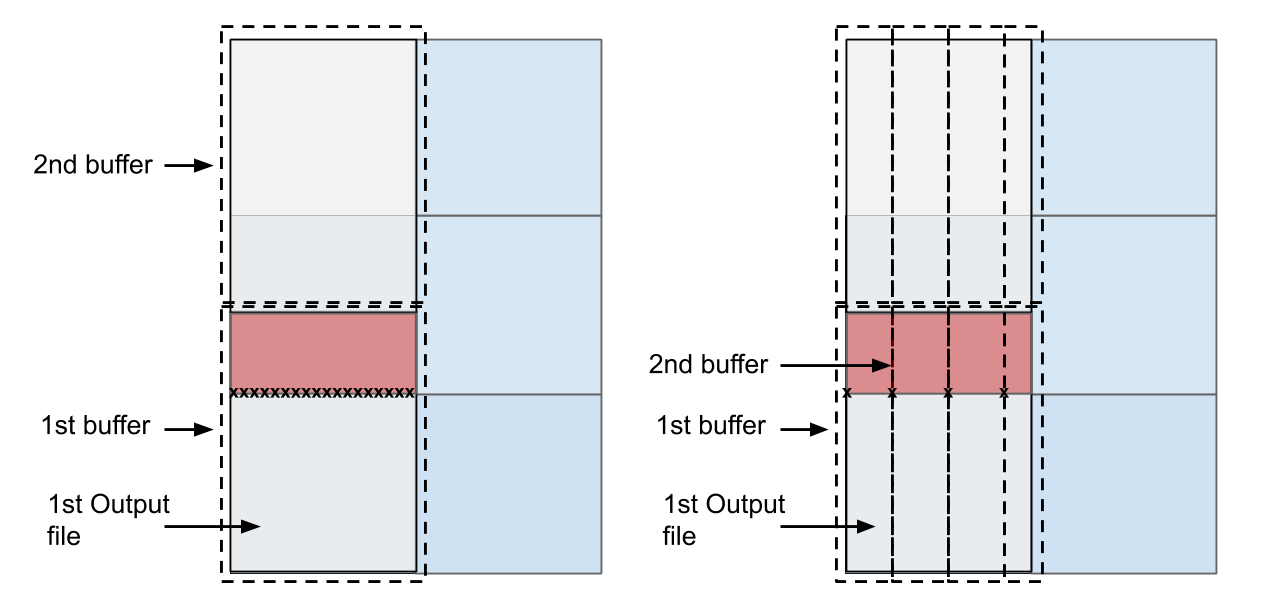
\includegraphics[scale=0.20]{./figures/case_1_2.png}
\caption{Left figure: without keep strategy.
Right: with keep strategy.
Keeping extra data in memory reduces the number of seeks caused by writing but increases the number of buffers needed to write an output file.
The crosses represent the number of seeks that happen in both cases.
}
\label{fig:case_1_2}
\end{figure*}

\begin{figure*}[h]
\centering
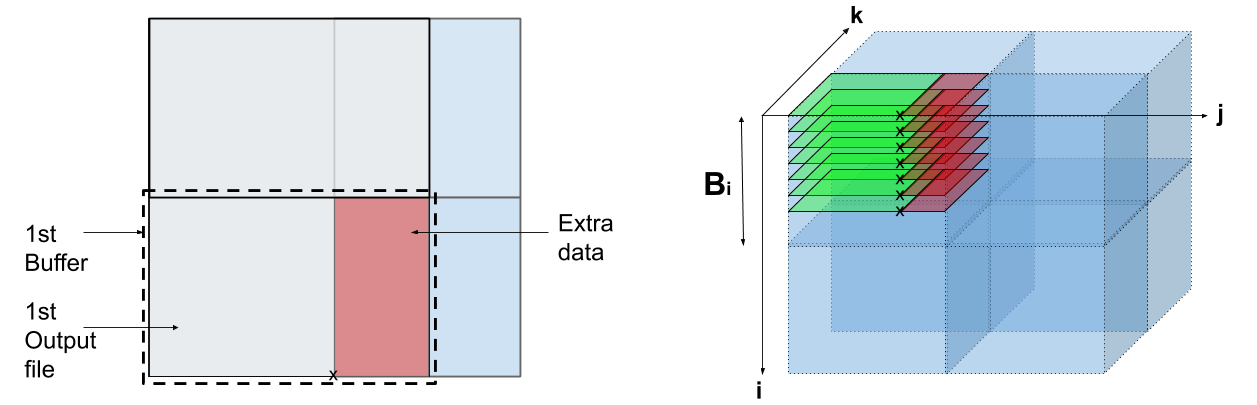
\includegraphics[scale=0.20]{./figures/case_2_1.png}
\caption{Illustration of an overlap in the $j$ dimension. The black crosses represents one seek each. In the 2D case on the left we can see that writing down the data into the next output file on the right would take only one seek. In the 3D case however (right side), writing the data down into the next output file would take $B_i$ seeks.
}
\label{fig:case_2_1}
\end{figure*}

Let us first consider the 2D case in which the input and output files overlap in one dimension only.
An overlap occuring in the $k$ dimension would incur $B_k$ seeks as opposed to 1 seek only (see Figure \ref{fig:case_1_2}) in the case of an overlap in the $j$ dimension (see Figure \ref{fig:case_2_1}).
Note that the keep strategy is not useful if we cannot store the extra data in one direction completely (see Figure \ref{fig:case_2_1}). \\

Let us define 3 overlaping areas, represented in Figure \ref{fig:areasabc}.
The $a$ area is the overlap in the $k$ axis.
The $b$ area is the upper right overlap which combines the overlaps in both axis.
One can see the $b$ area as the continuity of the $a$ area.
The $c$ area is the overlap in the $j$ axis only.
The $a$ area becomes the $A$ volume in 3D, the $B$ volume corresponds to the $b$ area, etc. \\

\begin{figure}[h]
\centering
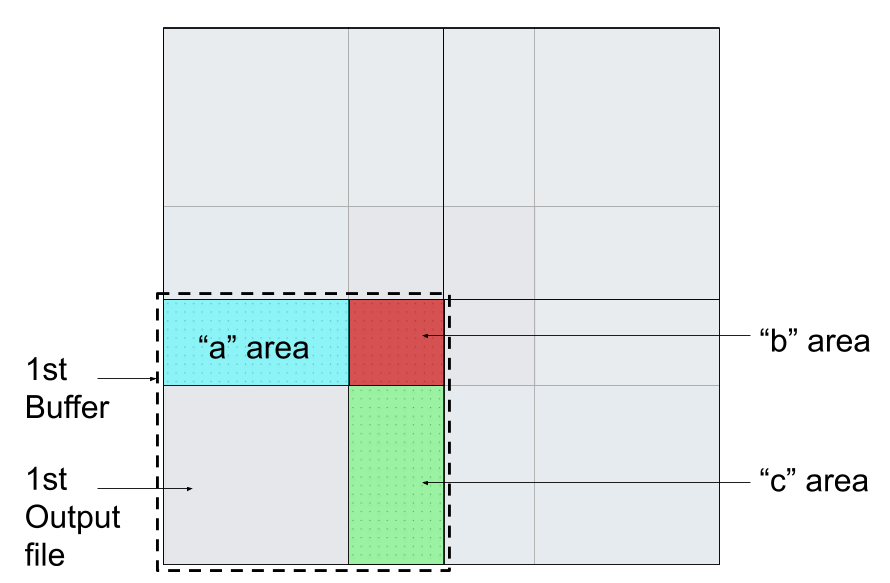
\includegraphics[scale=0.20]{./figures/areasabc.png}
\caption{Illustration of the different overlaping areas in 2D.
The blue area is called the $a$ area, the red area is called the $b$ area and we call $c$ area the green one.
}
\label{fig:areasabc}
\end{figure}

In terms of the number of seeks, $$\Omega_j > (\Lambda_j-\Omega_j) > 1 => \textrm{seeksIn(a)} > \textrm{seeksIn(b)} > \textrm{seeksIn(c)}$$ in 2D, and this stays true when increasing the number of dimensions.
We must therefore use the memory available for stretching the buffer to store $a$ first, then $b$, and finally $c$.
The same way that it is not useful to save part of the $c$ area as opposed to storing the whole $c$ area, it is not useful to inrease $B_j$ if $B_k < \Lambda_k$.
Indeed, the number of seeks will be the same than without using the keep strategy.
As the $b$ area is the continuity of the $a$ area in the $j$ direction, if the available buffer memory $m'$ allows to store the $b$ area but not the $b$ and $c$ areas together it seems that increasing $B_j$ from $\Omega_j$ to $\Lambda_j$ while storing only the $b$ area could save a lot of seeks. \\

As a conclusion, we should increase the fastest moving dimension first to allow the reduction of the number of seeks in the $a$ and $b$ areas in the $k$ direction.
Then we should increase $B_j$ as much as possible, while saving only $a$ and then $b$, even if we cannot cover it entirely.
Finally, if we can store the whole $c$ area, we should do it before inreasing the $i$ dimension to prevent the 1 seek to be multiplied by $B_i$. \\

\subsection{Stretching beyond the input aggregate shape}
Using small input and output file shapes, it is probable for the buffer to have been stretched to the input aggregate, which means that a good amount of RAM is still available.
One have no reason to stop increasing the shape of the buffer from that point.
The first idea which comes to mind is to stretch the buffer such that the buffer length becomes a multiple of the output file length in a given dimension $x$: $B_x = nO_x$.
Again, this would create an overlap in the input files however, which would prevent the keep strategy to be applied and create a maximum number of seeks.
Therefore, one can only stretch the buffer by adding one input file length to a given dimension of the buffer shape (see Figure \ref{fig:extendingbuffers}).
A good idea seems to be to extend the buffer shape in the dimension of the biggest overlap area/volume such that we accumulate extra data from the smallest overlap volumes only.
Again, if we can stretch the buffer such that $B_x = R_x$ in the dimension $x$ of the biggest overlap area/volume, we then increase in the dimension of the second biggest overlap size, etc.

\begin{figure*}[h]
\centering
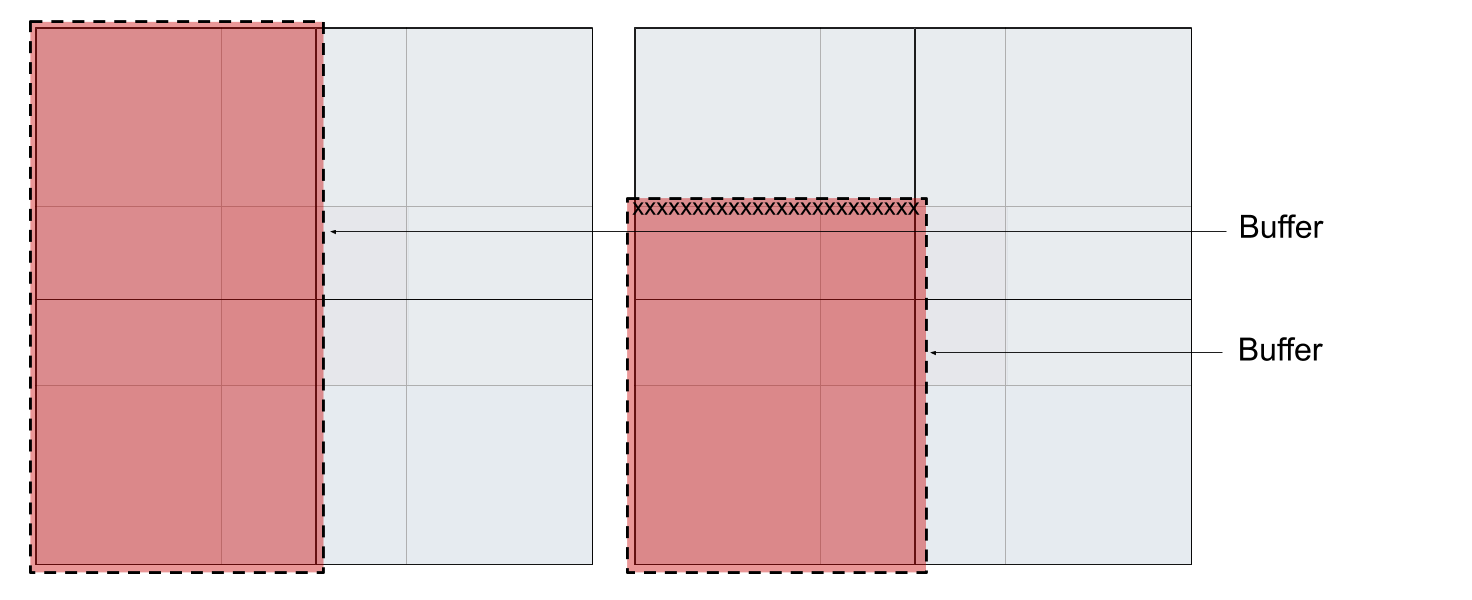
\includegraphics[scale=0.20]{./figures/extendingbuffers.png}
\caption{ Left side: Extending the buffer to the next input length. Right side: Extending the buffer to the next output length. The crosses indicates the number of seeks. As we can see, extending the buffer to the next output shape incurs a lot of seeks in the next input file when loading the buffer. As the input file is incomplete, there is no extra data, therefore the keep strategy cannot be used.
}
\label{fig:extendingbuffers}
\end{figure*}

\subsection{Pseudo-code of the algorithm}
The algorithm is described in Algorithm \ref{algo:getbuffershape}. \\

Details:
\begin{itemize}
  \item line 15: sort the axes in decreasing order of overlap cuboid size
  \item line 16: for each dimension in this order, try to increase the buffer size
  \item lines 17, 18: keep adding the length of an input aggregate in that dimension while there is memory left.
\end{itemize}

Nomenclature:
\begin{itemize}
  \item $A_i$: Area of the $i^{th}$ component
  \item $m$: Amount of main memory available for the buffer at initialization
  \item $m'$: Amount of main memory available for the buffer during the algorithm execution
  \item $\textrm{iterable}[i]$: Access the $i^{th}$ element of an iterable
  \item $B = (B_i, B_j, B_k)$: Shape of the buffer
  \item $(B_i B_j B_k)$: Size of the buffer in voxels
  \item $R_i, R_j, R_k$: Length of the reconstructed image in the $i^{th}$ dimension
  \item $I_i, I_j, I_k$: Length of an input file in the $i^{th}$ dimension
  \item $O_i, O_j, O_k$: Length of an output file in the $i^{th}$ dimension
  \item $C_i(x), C_j(x), C_k(x)$: Overlap size in voxels in the $i^{th}$ dimension, when loading the $t^{th}$ buffer.
  \item $\Lambda_i, \Lambda_j, \Lambda_k$: Length of an input aggregate in the $i^{th}$ dimension
  \item $\Omega_i, \Omega_j, \Omega_k$: Length of an output aggregate in the $i^{th}$ dimension
  \item $b_i, b_j, b_k = \frac{R_i}{B_i}$: The number of buffers in the $i^{th}$ dimension in the reconstructed image
  \item $f_1, f_2, f_3$: Names of the overlap areas in 2D
  \item $F_1, F_2, F_3, F_4$: Names of the overlap volumes in 3D
  \item $ N_s $: Number of buffers in a slice
  \item $ n_s $: Number of buffers read so far from the current slice.
\end{itemize}

\begin{algorithm}[h]
  \caption{getBufferShape in ND}

  \begin{algorithmic}[1]

    \STATE \textbf{INPUTS}: $m$, $\Lambda$, $B$

    \STATE $m' \gets m$

    \FOR {$d$ in $dims$}
      \IF{$m' >= \textrm{maxMemoryCost}(\textrm{B}.add(\Lambda_{dim}), dim)$}
        \STATE $\textrm{B.append}(\Lambda_{dim})$
      \ENDIF
      \IF{$\textrm{maxMemoryCost}(...\textrm{B}, 1) <= m' < \textrm{maxMemoryCost}(\textrm{B}.add(\Lambda_{dim}, dim)$}
        \STATE $maxnbcols = \frac{m'}{\textrm{cost}}$
	      \STATE $\textrm{buffershape.append}(maxnbcols)$
      \ENDIF
      \IF{$m' < \textrm{maxMemoryCost}(\textrm{B}.add(1, dim)$}
        \STATE $\textrm{nb dims so far = (dim - 1)}$
        \STATE $\textrm{nb dims left = nbdims - nb dims so far}$
        \STATE $\textrm{buffershape} = \textrm{buffershape} + \textrm{ones(nbDimsLeft)}$
      \ENDIF
    \ENDFOR

    \STATE $\textrm{maxIndexes = sortIndexOfMaximumFall(B)}$ % get axis of maximum overlap
    \FOR{$maxIndex$ in $maxIndexes$}
      \WHILE{$m' > \textrm{maxMemoryCost}(\textrm{B}.add(\Lambda_{maxIndex}), maxIndex)$}
        \STATE $\textrm{B[maxIndex]} += \Lambda_{maxIndex}$
      \ENDWHILE
    \ENDFOR

  \end{algorithmic}
  \label{algo:getbuffershape}

\end{algorithm}

\subsection{Special case of non optimality}
When the amount of memory available is too small, a special case arise where the algorithm is not optimal.
Consider the 2D case where there is an overlap in the $k$ dimension only (see Figure \ref{fig:case_1_2}).
Let us say that the buffer size is such that $B_k = \Lambda_k$, but is too small to extend $B_j$ to $\Lambda_j$.
Keeping the extra data from the overlap in the $k$ dimension in memory allows us to write contiguously in the output files but it implies using more buffers in the $j^{th}$ axis.
In the worst case, $B_j = 1$ which incurs $\Lambda_j$ seeks.
As soon as $B_j > 1$ however (keeping $B_k = \Lambda_k$), we divide the number of seeks produced by writing in the incomplete output file per the number of buffers.
This observation is true for the other dimensions as well: as soon as $B_x = \Lambda_x$ in a given dimension $x$, the more we can read in the next dimension $x+1$, the better.
This proves that we should not increase a dimension if $B_x < \Lambda_x$ in the preceeding dimensions.

\subsection{Impact of the buffer order on performance}
Using the keep strategy in case of overlaps, one may order the buffer loadings to further reduce the number of seeks.
By optimizing the buffer ordering one can reduce the maximum quantity used to store the extra data in memory.
For example, if an overlap occurs only in the $k$ axis, loading the next buffers in this direction will enable recycling the extra data kept in memory, resulting in a smallest memory consumption over time.
The memory saved thanks to a smart ordering could enable the storage of more overlaps in memory using the ``keep strategy", further reducing the overall number of seeks. \\

\begin{figure*}[h]
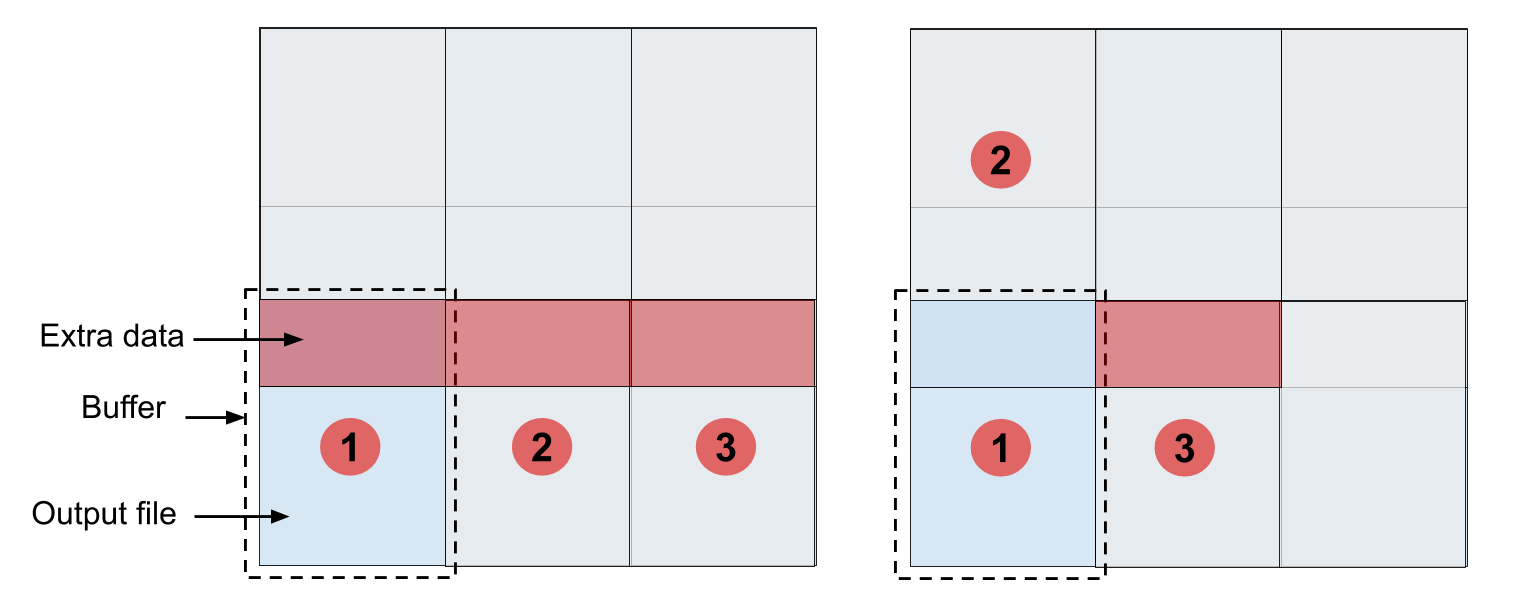
\includegraphics[scale=0.2]{./figures/goodorderingbadordering.png}
\caption{ Comparison of a bad buffer ordering (left side) against a good buffer ordering (right side), given an overlap in the $k$ dimension.
The red area represents the amount of extra data kept in memory after loading the third buffer.
The right side order allowed to release the extra data from the first buffer after reading the second buffer.
}
\label{fig:goodorderingbadordering}
\end{figure*}

As we will see, the buffer ordering problem is complex and does not seem easily solvable.
Thanksfully, the impact of the buffer ordering on performance can be mitigated.
Indeed, the impact of the buffer ordering depends on the size of the falls, i.e. the overlaps between the buffer and the incomplete output files' shapes.
One can reduce the falls' sizes by using smallest chunks:
Even if the overlap between the input and output files is big with respect to their size, the area/volume of the falls will be kept small.
In particular, we remark that the falls tends to be smaller when the buffer shape is bigger than the output file shape, as the overlaps are smallest and concentrated on the borders (see Figure \ref{fig:goodorderingbadordering}).
We can stimulate this property by using small chunks such that we use buffer bigger input aggregates (see Stretching beyond the input aggregate shape), while keeping the overlaps small at the borders.

%----------------------------------------
\section*{A memory analysis}
%----------------------------------------

The keep algorithm assumes that $m$ is big enough to keep at least a ``complete column" of length $B_k$.
As it has been explained, the buffer is then stretched in the $j^{th}$ dimension and so on as long as there is enough main memory available to use the keep strategy.
This section covers how we estimate the amount of memory required by the keep strategy in order to know how much we can stretch the buffer in one dimension at a time. \\

According to the ``keep" algorithm, the buffer is stretched in the storage order.
As a consequence, only a set of possible overlaps may happen, as illustrated on Figure x.
In order to compute the maximum amount of memory required by the keep strategy given a specific buffer shape, we must proceed as follows:
\begin{itemize}
  \item 1) Given a buffer shape, identify the current case among those presented on Figure x. For each case we shall define a formula that computes the amount of extra data when loading a given buffer at step $s$.
  \item 2) Compute the maximum overlap length in all dimensions.
  \item 3) Compute the worst case in terms of memory consumption, according to the buffer ordering.
\end{itemize}

\subsection{A ``naive" buffer ordering algorithm}
The buffer order defines the maximum amount of extra data we will have to keep in memory.
As we do not know a good ordering which do not imply a compute-intensive algorithm (see section ``Discussion"), let us define a naive ordering as follows (Algorithm \ref{algo:naivebufferordering}):

\begin{algorithm}[H]
  \caption{Naive buffer ordering algorithm}
  \begin{algorithmic}[1]
  \STATE \textbf{INPUTS}: inputShape, outputShape
  \STATE $overlap \leftarrow dict()$
  \STATE $overlap \leftarrow \textrm{getOverlapUpperBounds(\textrm{inputShape, outputShape})}$
  \STATE $\textrm{sort(overlap, by=values)}$
  \RETURN $\textrm{overlap.keys()}$

  \end{algorithmic}
  \label{algo:naivebufferordering}
\end{algorithm}

The algorithm returns an array of dimension indices, ordered by decreasing overlap size.
The idea is to read the buffers in the first direction where the overlap is the most important, then the second etc.
For example if the order is (j, k, i), we will read the buffers in direction j first (see figure x).
We evaluate the amount of overlap thanks to the function $\textrm{getOverlapUpperBounds}$.
$\textrm{getOverlapUpperBounds}$ returns, for each dimension, the amount of memory needed to keep the extra data in memory if we read a buffer row (a row of buffers in the reconstructed image) in this dimension. \\

\subsection{Computing the overlap size in 3D}
% figure of $b_x$

In a given dimension $x$, when loading the $n^{th}$ buffer, the overlap length is $C_x(n) = nB_x mod (O_x)$ with $i \in [1, b_x]$ where $b_x$ is the number of buffers in the direction $x$.

% figure of the overlap sizes (could reuse the overlapsabc and just adding the sizes)

In 2D, the size of the overlap is:
\begin{itemize}
  \item $C_k(x)B_j$ while the $a$ and $b$ areas are not totally covered by the buffer ($B_j < \Lambda_j$).
  \item The sum of the sizes of the $a$, $b$ and $c$ areas:
  \begin{itemize}
    \item Size of the b area: $C_k(x)(B_j-C_j(y))$
    \item Size of the b area: $C_k(x)C_j(y)$
    \item Size of the c area: $C_j(y)(B_k-C_k(x))$
  \end{itemize}
\end{itemize}

% \subsection{Computing the overlap size in the 3D case}
% In this analysis we express the overlap size in terms of the number of voxels that constitutes the overlap because the real quantity of memory used depends on the size of a voxel in memory.
% For convenience one can avoid this extra parameter by setting the number of bytes per voxel to 1. \\
%
% When loading the first buffer in a given dimension $i$, the overlap length $C_{x}(1)$ (value of $C_x$ when loading the first buffer) is $B_x \mod O_x$ by definition of an output aggregate (see Figure x).
% When loading the $i^{th}$ buffer, the overlap length is therefore $C_{x}(i) = i * B_x \mod O_x$ with $i \in [1, b_x]$ ($b_x$ is the number of buffers in direction $x$).
% Let us call the index of the buffer in dimension $k$, $j$, $i$: $x$, $y$ and $z$ respectively. \\
%
% In two dimensions, there are three overlap areas: $a$, $b$ and $c$. When we are loading the $(x, y)^{th}$ buffer, the $x^{th}$ buffer in dimension $k$ which is also the $y^{th}$ buffer in dimension $j$, the overlap size in voxels is:
% \begin{itemize}
%   \item $a = C_k(x) * (B_j - C_j(y))$ ($C_k(x)$ is the length of the overlap in direction $k$ for the $k^{th}$ buffer)
%   \item $b = C_k(x) * C_j(y)$
%   \item $c = C_j(y) * (B_k - C_k(x))$
% \end{itemize}
%
% According to the algorithm, $c$ can be kept in memory by the keep strategy only if there is enough memory to store $a$ and $b$.
% The same way, $b$ is kept in memory only if we can keep $a$ before.
% When stretching the buffer shape, we start by adding as much rows as possible in the first moving direction, then the second one until we can keep b entirely,
% Keep in mind that c can only be stored completely, or it is not stored, as storing it only saves 1 seek.
%
% \begin{figure*}[h!]
% \centering
% 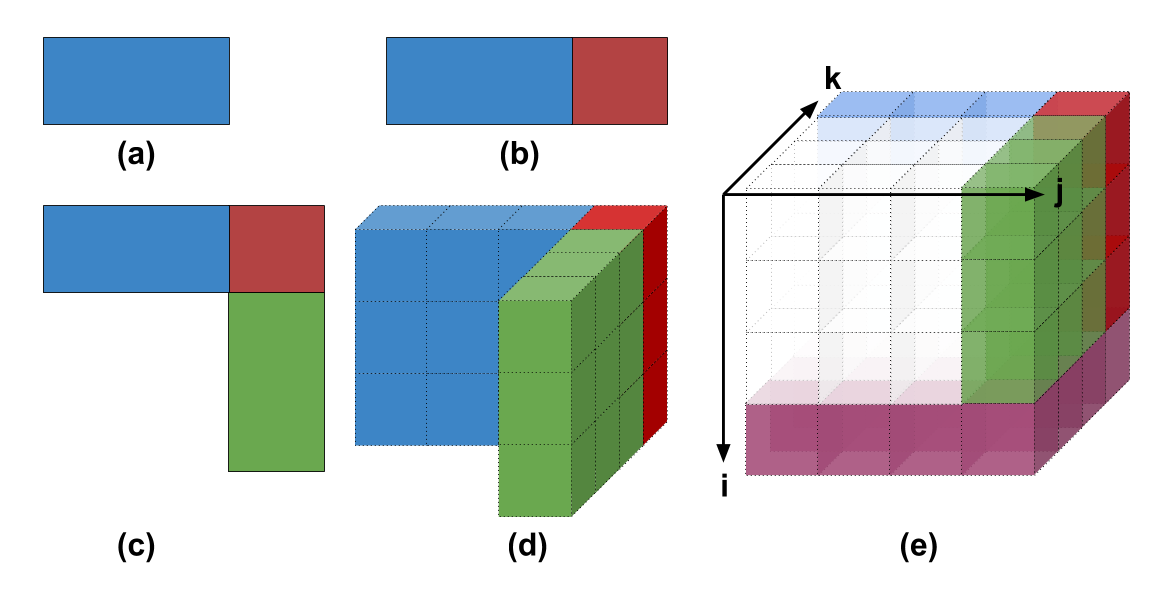
\includegraphics[scale=0.3]{./figures/overlapsin3d.png}
% \caption{Possible overlaps when resplitting 3D images.
% (a): Covering the $a$ area.
% (b): Covering the $b$ area.
% (c): Covering the $c$ area.
% (d): Converting overlap areas into overlap volumes by stretching the buffer in the $i$ direction.
% (e): Further increasing $B_i$ creates a $d$ overlap volume.
% }
% \label{fig:overlapsin3d}
% \end{figure*}
%
% In 2D, the overlap area in number of pixels is either (see Figure \ref{fig:overlapsin3d}):
% \begin{itemize}
%   \item $\textrm{overlap} = C_k(x) * B_j$ if we keep only $a$ in memory.
%   \item $\textrm{overlap} = C_k(x) * B_j$ if we keep $a$ in memory as well as $b$ or a part of $b$.
%   \item $\textrm{overlap} = a + b + c$ as defined above i.e. we store c completely.
% \end{itemize}
%
% In 3D (see same Figure x), the overlap area is first increased into an overlap volume:
% $\textrm{overlap} = (a + b + c) * B_i$ if we cannot store $d$ completely.
% Then, if $B_i = \Lambda_i$ we add the whole $d$ volume directly.
% The overlap area is therefore:
% $$\textrm{overlap} = [(a + b + c) * (B_i - C_j(z))] + d_{\textrm{volume}}$$, with
% $$d_{\textrm{volume}} = C_j(z) * C_j(y) * C_k(x)$$
%
% \subsection{Computing the maximum amount of memory needed for the keep strategy}
%
% \noindent \textbf{Maximum length of the overlap in a given dimension} \\
% By definition of the modulo, the maximum overlap length in a given dimension $x$ is $O_x$.
% $O_x$ is an upper bound as in some cases like in Figure x we may never reach this point.
% We could therefore compute $k * B_x \mod O_x$ for all $k \in [1, b_x]$ to find the maximum if it is not too compute intensive in order to find the exact maximum length of the overlap in direction $x$. \\
%
% \noindent \textbf{Maximum overlap size} \\
% Now that we know how to compute the maximum length of the overlap, we can use the overlap sizes found in section ``Computing the overlap size in the 3D case" and replace the $C$s by their maximum value to get the maximum volumes we can expect for $a$, $b$, $c$ and $d$ during the algorithm's execution.
% Given a buffer ordering, we may have to store several times one or more volumes at the same time in memory. \\
%
% \noindent \textbf{Total overlap size at a given time} \\
%
% Using the naive ordering, we read buffers in the direction of the biggest overlap volume first.
% For example, if the buffer shape is the same as the shape of the input aggregate and if $volumes(k) > volumes(j) > volumes(i)$, then we read the buffers in the $k$ direction first.
% The amount of memory needed to read in the $k$ direction is $m_{\textrm{needed}} = B.size + volumes(k)$:
%
% \begin{itemize}
%   \item At step $t = 1$, the first buffer is read, and there is no preceeding overlap.
%   \item At step $t > 1$, we have the $C_k(t-1)$ overlap in main memory. We need to read the $t^{th}$ buffer first in order to get rid of the previous overlap and store the new one.
%   \item The last buffer being read in the $k$ direction has no overlap by definition of the resplit process: everything is written down, including the previous overlap $C_k(t-1)$.
% \end{itemize}
%
% \begin{figure}[h!]
% \centering
% 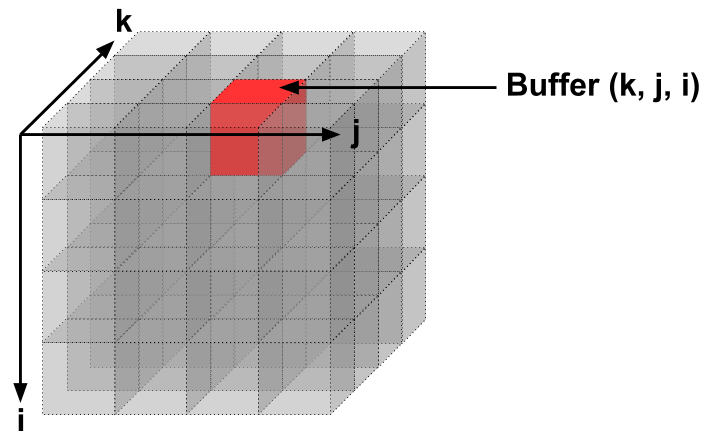
\includegraphics[scale=0.3]{./figures/bufferkji.png}
% \caption{Buffer in position (k,j,i) in the referential of the buffers.
% \label{fig:bufferkji}
% }
% \end{figure}
%
% During the buffering process in direction $k$, we must store the overlap volumes in the $j$ and $i$ directions, too, according to the keep strategy in order not to write it down which would incur a lot of seeks.
% In 3D, when loading the buffer in position (k, j, i) in the referential of the buffers (see Figure \ref{fig:bufferkji}), the overlap size is:
% $$ MAX =  bufferSize + C_k(x) + [kC_j(y) + (n_k-k)*C_j(j-1)] + [n_s*C_j(z) + (N_s - n_s)*C_j(z)] $$
%
% \begin{itemize}
%   \item $N_s$ is the number of buffers in a slice.
%   \item $n_s$ is the number of buffers read so far from the current slice.
% \end{itemize}
%
% \noindent \textbf{Maximum amount of memory needed for the process} \\
% Defining $x_{max}$ and $y_{max}$ the index at which we are storing the biggest overlap in $k$ axis and the index of the buffer row at which there is the biggest overlap in $j$, respectively, we know that the case $(x_{max}, y_{max})$ will happen.
% The same way, the case $(x_{max}, y_{max}, z_{max})$ will also happen.
% Therefore, the maximum memory size we will need during the whole process is $MAX$ with all $C$ replaced by their maximum possible value: either the upper bound or the computed value as explained in the preceeding paragraph.

%----------------------------------------
\section*{Implementation}
%----------------------------------------

%----------------------------------------
\section*{Experiments}
%----------------------------------------

%----------------------------------------
\section*{Discussion}
%----------------------------------------

\subsection{Comparison with previous work}
\subsection{Solution of the ordering problem}
\subsection{Extending the algorithm for ROI extraction}
\subsection{Distributed keep algorithm}

%
% \subsection{Solution of the ordering problem}
%
% Our goal is to order the buffers so that we use the least memory as possible through the entire resplit process.
% In other words, we want to minimize the maximum amount of main memory used during the respit. \\
%
% \subsubsection{Memory deltas}
% One can model the sequential buffer loading problem as a doubly linked directed complete graph where each node is a buffer.
% Exchanges of data happen in main memory as we walk sequentially through the nodes using the ``keep strategy":
% At each node we get rid of some extra data loaded from previous buffers and we get some extra data from the new buffer.
% We call this difference between the amount of data in main memory before and after passing through a node a ``memory delta". \\
%
% \subsubsection{Modeling the problem as a shortest path problem}
% We will prove in the next paragraph that minimizing the maximum amount of memory during the resplit process is equivalent to finding the shortest path through all nodes of the previously defined graph with the ``distance" (weight on the edges between nodes) being the memory deltas.
% The algorithm must go through each node only once as we want to load all the buffers, only once (due to the non-overlaping buffer constraint).
% Note that weights can be negative if we give more extra data than we receive at a given node.
% Also note that weights update each time a buffer has been loaded:
% All the buffers that will recycle the extra memory from the current buffer see the weights of their incoming edges decrease. \\
%
% \subsubsection{Minimizing the maximum amount of memory is equivalent to a shortest path problem}
% The idea of the proof is that if the solution of one problem is the solution of the other, then they are be equivalent. \\
% To do. \\
% Note to self: An optimal solution of the shortest path problem with memory deltas as distances is a path that minimizes the sum of the memory deltas encountered during the process.
% % figure showing the sequence and the different cases
% Let us take such an optimal path and consider a sequence of the main memory used at each step on the path. \\
%
% \subsubsection{Conclusion}
% The buffer ordering problem is an all-pairs (we can start from any node and and at any node) dynamic (the weights update during the process) shortest-path problem.
% According to a review by Madkour et al.\cite{shorestpathsurvey}, Demetrescu and Italiano proposed a ``Fully dynamic algorithm over directed graphs for all-pairs shortest-paths with real-valued edge weights"\cite{demetrescu} to solve such a problem.
% Their solution seems to have been improved by Thorup in his paper ``Fully-Dynamic All-Pairs Shortest Paths: Faster and Allowing Negative Cycles"\cite{thorup}.
% The amortized update time is $O(n^2log^3(n))$ which is not a small overhead (Book of algorithm theory 2004).
% Proving the benefit of using such an algorithm reveals to be a complex time, that is why we decide to leave it as a future work and use a naive buffer ordering for the moment.
%
% \subsection{Comparison with previous work}
%
% \subsubsection{Split behavior of the algorithm}
% The split process is equivalent to the resplit process with the special case of having only one input file.
% In this case, the input aggregate has the same shape than the reconstructed image.
% The buffer will first be stretched in the $k$ direction until $B_k = \Lambda_k = \textrm{R}_k$.
% Then we will stretch in the $j$ dimension until $B_j = \Lambda_j$ and the same behavior applies in the $i^{th}$ dimension.
% Therefore, we first store complete rows, then block row tiles, then slices, block rows and slices.
% This algorithm is identical to the ``multiple reads" algorithm (see Hayot-Sasson et al.).
%
% \subsubsection{Merge behavior of the algorithm}
% The merge process is equivalent to the resplit process with the special case of having only one output file.
% In this case, the input aggregate has the same shape than the output file shape.
% The buffer will be stretched in the $k$ axis until $B_k = \Lambda_k = \textrm{R}_k$.
% Again, this is the same behavior than multiple reads.

%----------------------------------------
\section*{Conclusion}
%----------------------------------------

%----------------------------------------
\section*{Acknowledgment}
%----------------------------------------

\bibliography{Bibliography}
\bibliographystyle{ieeetr}

\end{document}
